% \textcolor{blue}{
% \textbf{Deliverables:}
% \begin{itemize}
% \item requirements $\xrightarrow{\rm status}$ draft
% \item concept design (if necessary baseline and backups) including 3D model
% \item main questions to answer in this subsection
%     \begin{itemize}
%     \item number of coils
%     \item coil size
%     \item power consumption
%     \item envelope for inductance
%     \item active component?
%     \item minimum number of magnetometers
%     \item achievable sampling frequency, ...
%     \end{itemize}
% \item calculations proving that the design concept fulfills the requirements 
% \item interface definitions (detailed)
% \item design and manufacturing plan
% \item schedule
% a\end{itemize}
% }
\subsection{Overview}
The location of the nEDM spectrometer in an accelerator facility necessitates a system to reduce influences of environmental magnetic fields to the experiment. As mentioned in an earlier section [ref, MSR], there is a strong background field of $\approx 350\,\mu$T in the TUCAN area in the TRIUMF Meson Hall. The FEA simulations revealed that such a strong field could saturate the mu-metal layers of MSR, and worsen its shielding performance [ref, 9.4.1]. In addition, there are also occasional field perturbations on the order of $\sim 10\,\mu$T, which may require demagnetization procedures of MSR. 

The Ambient Magnetic-field Compensation (AMC) subsystem will consist of a set of coils and magnetometers to provide static and dynamic magnetic field compensation in the exterior of MSR to ensure the shielding performance of MSR and increase possible  up time of the EDM measurements. This section specifies the key requirements of this subsystem and some developmental works performed in this context.  

%\begin{figure}[htb]
%\centering
%%trim={<left> <lower> <right> <upper>}
%\includegraphics[width=0.99\textwidth, trim = {0cm 0cm 3cm 0cm},clip]{./graphics/AMC/figurename}
%\caption{.}
%\label{fig:SourceUCNhandlingcomponents}
%\end{figure}
%\begin{figure}[htb]
%\centering
%%trim={<left> <lower> <right> <upper>}
%\includegraphics[width=0.8\textwidth, trim = {5cm 0cm 6cm 0cm},clip]{./graphics/UCNHandlingEDM}
%\caption{}
%\label{fig:AMC-}
%\end{figure}




\subsection{Purposes}

The PSI nEDM experiment also employed a system of surrounding field compensation [Afach2014]. To compare the situations of the PSI nEDM and the TUCAN area in  TRIUMF Meson Hall, and to clarify the requirements in our case, typical numbers to characterize the magnetic environments are listed  in Table \ref{tab:amc_comparaion}. 

One significant difference between the two is the order-of-magnitude stronger static background field in the TUCAN area which is due to the stray field of the TRIUMF cyclotron. As long as this issue is well treated and the function of MSR secured, TUCAN MSR is expected to provide sufficient suppression of the background fluctuations to the order of $\sim10\,$pT in the averaging time of $\sim 100\,$s. 
Therefore, unlike the case of the PSI experiment where the active magnetic field compensation was used during the EDM measurement sequence to maintain required magnetic field stability, the active field control is not necessaryfor TUCAN during the EDM measurement sequence, except occasions when the field varies in steps on the order of $\sim 10\,\mu$T (see below).

In both cases, occasional strong magnetic field variations exist. In case of the PSI experiment, neighboring superconducting magnet test facilities were operated in daily bases,  producing magnetic field variations up to $30\,\mu$T. According to [Afach2014],  field variations of this order required a degaussing (or idealization) procedure of the passive shielding. The needs of this procedure, which typically took about 30\,min to an hour, were reduced by the active compensation suppressing them by a factor of $\approx10$ [Afach2014]. In case of TUCAN, an overhead bridge crane in the hall, which is operated typically once in a few days, is found to produce magnetic field variations on a comparable order. Therefore we should anticipate that such field variations will make degaussing procedures required. Active magnetic field compensation can possibly reduce the needs of degaussing procedures, if it can suppress some of the field variations to the order of $1\,\mu$T or below, it can even make the EDM measurement possible under such field variations.

Based on the above discussions, the purposes of the AMC are 
\begin{itemize}
    \item to provide static magnetic field compensation in order to prevent the background field of $\approx 350\,\mu$T from saturating MSR 
    \item to provide compensation of dynamic magnetic field. Its main target is the strong field variations on the order of $\sim 10\,\mu$T. This will increase potential up time of the EDM measurements. On-site tests in the commissioning phase of AMC should also be performed.
\end{itemize}

\begin{table}[hbt]
\centering 
\begin{tabular}{|l||c|c|}
\hline

 & \multicolumn{1}{c|}{\textbf{PSI}} & \multicolumn{1}{c|}{\textbf{TUCAN}} \\ \hline\hline 
Static background field  & $\approx62\,\mu$T & $\approx 350\,\mu$T                       \\ \hline
Background field fluctuations  $\sigma_{|\mathbf{B}|}(100\,\mathrm{s})$ & $\approx 1\,\mathrm{nT}$ (night), $\approx 80\,\mathrm{nT}$ (day) & $\lesssim 80\,\mathrm{nT}$ \\ \hline
Occasional variations    & $\lesssim30\,\mu$T   & $\lesssim 50\,\mu$T            \\ \hline
 MSR shielding  factor       &    $\sim 10^4$   &   $\sim 10^5$ (planned)  \\ \hline 
\end{tabular}
\caption{List of typical numbers characterizing the magnetic field environment of the PSI nEDM experimental site and the TUCAN area in TRIUMF Meson Hall. The table consists of typical values of: the static background field, the magnetic field fluctuations evaluated by the Allan deviation with an averaging time of 100\,s, typical amplitudes of occasional magnetic field variations, the quasi-static shielding factor of MSR. The values of the PSI experiment are based on [Afach2014, Franke2013]. Those of TUCAN are based on [Sarte2013] and recent measurements discussed in Section \ref{sec:amc_recent}. 
}
\label{tab:amc_comparaion}
\end{table}


\subsection{Requirements}
The key requirement specifications on the performance of AMC are stated below:

\begin{RSenumerate}[resume]
\item    The static magnetic field compensation of AMC should reduce the field surrounding MSR such that  $|\mathbf{B}|<0.1\,$T is satisfied in the mu-metal layers of MSR. \label{RS:amc_rs_sta}
\begin{itemize}
    \item[\textbf{Rationale:}]  The saturation magnetic induction of mu-metal is about $ 0.7\,$T. We require $|\mathbf{B}|<0.1\,$T  in order to have a large enough safety margin.
    \item[\textbf{Test:}] In defining the geometries of the coils, FEA simulations are essential which include a realistic background field, MSR, and the compensation coils to confirm that the requirement is satisfied. 
\end{itemize}

 \item The dynamic compensation of AMC should compensate the external field variations on the  order of $\sim 10\,\mu$T by a factor of $\approx 10$ when they are experienced by MSR. \label{RS:amc_rs_dyn}
 \begin{itemize}
    \item[\textbf{Rationale:}] 
    There are not many preceding studies discusssing the threshold above which  a given shield needs deguassing. However, the reduction of a factor $\sim 10$ would significantly lessen the influence of the perturbations to MSR. This is also a realistic aim, regarding the preceding work by PSI [Afach 2014]. 
    \item[\textbf{Test:}] 
    To achieve this, the spatial and time properties of the target magnetic field variations are important factors. The coils should be designed based on the measured properties. 
\end{itemize}

  \item The target of the static and dynamic compensation of AMC should include  a  volume which contains the parts of MSR which are moved by opening or closing of the door of MSR [ref, figure in MSR section]\label{RS:amc_rs_volume}
 \begin{itemize}
    \item[\textbf{Rationale:}] In order to prevent saturation of these parts.  This will be required for operation as well as commissioning of MSR. 
\end{itemize}
\end{RSenumerate}

The AMC subsystem is still in the phase of concept design, therefore its hardware requirements have not been clarified yet. 
They should include, for example, space requirements in order not to interfere the other subsystems, the response times of the system which would constrain the inductances of the coils and switching times of the power supplies, and an adequate rate and accuracy for the readout of the magnetometers. They will be detailed as the design work proceeds. 


\subsubsection{Status of the concept design}
In the following, recent developmental works performed for the design of AMC are summarized. 

\subsubsection*{Feasibility check of the static compensation}
\begin{figure}[htb]
    \centering
    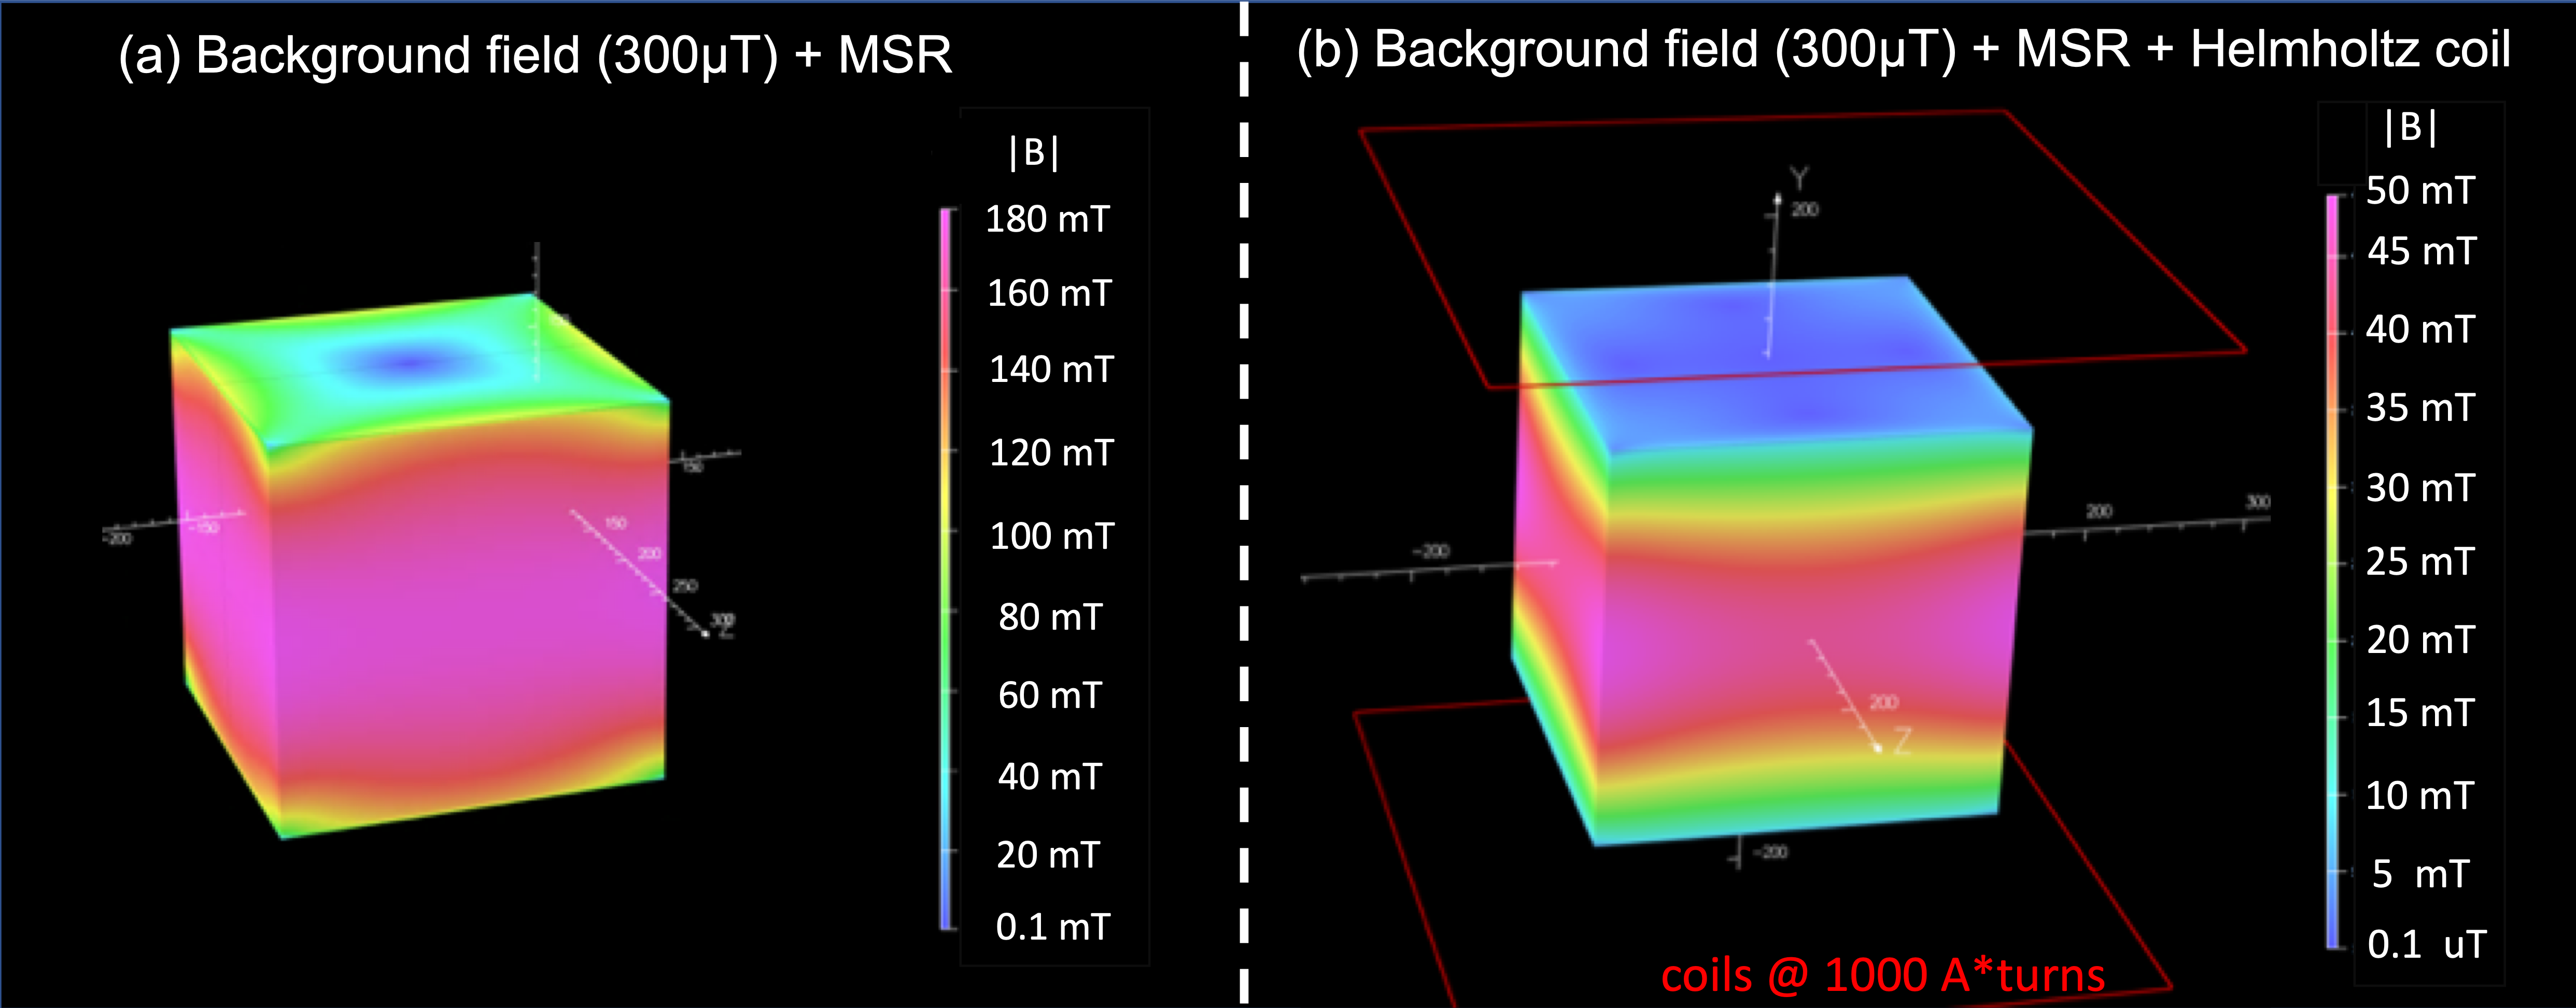
\includegraphics[width=\textwidth]{graphics/AMC/feasibility.png}
    \caption{FEA simulations to confirm the feasibility of the static compensation to prevent saturation of mu-metal layers of MSR. (a) A two-layer mu-metal box with the outer layer size of 2.34\,m x 2.34\,m x 2.34\,m is placed in a homogeneous background magnetic field. The background field has a strength of  $300 \mu$T and directed along the vertical axis of the model. The field resulted in the outer mu-metal layer is at maximum $180\,$mT. (b) A Helmholtz coil pair (each coil with a size 4\,m x 4\,m, placed apart by 3.8\,m) with 1000 A$\cdot$turns is added to the model of (a). It can be seen that the field in the outer mu-metal layer is reduced to $<50\,$mT.    }
    \label{fig:amc_feasibility}
\end{figure}
Shown in Fig.\,\ref{fig:amc_feasibility} is results of FEA simulations performed to confirm the feasibility of the static compensation of a background field on the order of $\sim 100\,\mu$T. In Fig.\,\ref{fig:amc_feasibility}\,(a), a two-layer cube  of mu-metal representing MSR is placed in a homogeneous background field of $300\,\mu$T. 



\subsubsection*{Recent magnetic field measurements in Meson Hall}\label{sec:amc_recent}
(explain the motivations, show the map and coordinate definition)
\subsubsection*{Characterization of the static background field}
(show the plots, above $\sim$1 m from the floor, the z component is almost constant)
\subsubsection*{Characterization of the field variations caused by the overhead crane}
(Crane variations characterized by sensors fixed at multiple locations
\begin{itemize}
    \item Field variations created by bridge is homogeneous (<1muT/m) and not so large < 10muT
    \item Field near the hook even goes up to 100 $\mu$T for the nearest sensor (**m?)
\end{itemize}
As the variations of the crane is one of the main target of the dynamic compensation, these characterizations will be considered in designing the coils for dynamic compensation.)
%\begin{table}[tb]
%\centering
%\caption{Parameters characterizing the magnetic environment of the TUCAN apparatus in the TRIUMF Meson Hall, listed in comparison of those of PSI-nEDM experiment.  [Afash]
%Magnetic field environment in TRIUMF Meson Hall in comparison to PSI-nEDM experiment. }\label{tab:MSR-comparison}
%\vspace{1em}
%\begin{tabular}{|l|c|c|}
%\hline
% & TUCAN  & PSI-nEDM \\ \hline \hline 
%Static background field strength $ |B|$ & $\approx 350\,\mu$T  & $\approx 62\,\mu$T \\ \hline
%Fluctuations (@100\,s averaging) & $ \lesssim 100$\,nT & $\sim100\,$nT  \\ \hline
%Occasional variations & $ \lesssim 30\,\mu$T (crane) & $ \lesssim  30\,\mu$T     (SULTAN/EDIPO)    \\ \hline
%MSR quasi-static shielding factor  &  $\sim 10^5$ & $\sim 10^4$ \\ \hline 
%\end{tabular}
%\end{table}




\subsection{Timeline}
(aiming to complete concept design by March 2020)



% \subsection{DAQ/AMC Interface Requirements}

% Q1: Will your subsystem be providing a data stream (over some network connection) to the DAQ/controls?  Or will you be providing an analog signal(s) that you want digitized by some DAQ/controls module? 
% If you are providing only a data stream, then you can skip question 2.

% A1: The AMC will provide a data stream


% Q3: Does your subsystem require a digitizer that is referenced to a central atomic clock?

% A3: No. The subsystem acquires magnetic field data and makes response to it of necessary, but it is not required to synchronize this process to an external clock with extreme precision. The status of the system, such as recorded magnetic fields or currents set to coils will be recorded to MIDAS as for the other subsystems, but moderate precision of the absolute time is sufficient for this purpose, too.

% Q4: Does your subsystem have controls or gas handling like equipment?


% Q4.1 If yes does your equipment require PLC-type interlocks to ensure correct/reliable operation?  Ie is there equipment-protection, safety or operational reasons why controls needs to be done with a PLC-type system? Or is it sufficient to have a computer program doing the control?

% A4: The control of the subsystem can be decided later, but seems to be ideal to use EPICS/MIDAS as for the other parts of the experiment. No gas handling like equipment is planned to be included in this  subsystem.

% \begin{thebibliography}{9}
% \bibitem{Afach2015}
% Afach 2015

% \end{thebibliography}


\begin{center}
\textcolor{blue}{
------------------------------[Old draft ]--------------------------------------------
}
\end{center}







\paragraph*{RS 3.-34}	The AMC shall reduce the external magnetic field to a level comparable to Earth magnetic field, less than 50 muT 
\newline Rationale: 	
%The passive shielding of the MSR can only handle a field of a certain magnitude, so the external field must be compensated.
We do not expect the outer layer of the MSR to saturate (refer to A Sher's calulations to be inserted into this document), however, the manufacturer of the MSR will not certify it's performance for any external field value larger than Earth field
\newline Rationale: 	The 50 muT requirement is Earth’s field, but a smaller target field may be desirable
\paragraph*{RS 3.-35}	The AMC shall be constructed in such a way that it does not prevent access to the MSR. A 'door' as well as a roof lid might be required in the AMC coil cage.
\newline Rationale: 	It will certainly be necessary to enter the MSR throughout the experimental run, so the AMC cannot render this impossible.
\paragraph*{RS 3.-36}	The ambient field of the experimental area shall be mapped and monitored to a precision acceptable to specify the construction of the AMC; 
\newline Rationale: 	It is important to understand the ambient magnetic conditions due to other magnetic equipment prior to running the experiment. ie the maximum DC values and amplitude of AC changes need to be known such that the right power and bandwith/speed of power supplies as well as inductance of coils can be chosen/determined.
\paragraph*{RS 3.-37}	The ambient magnetic field control system shall be developed such that its cost falls within the CFI budget allocation.
\newline Rationale: 	 This is necessary for completion of the experiment.
\paragraph*{RS 3.-38}	Development of the ambient magnetic field control systems shall be completed in the timeframe given by the Level 1 schedule shown in Document-154393. Critically this specifies installation of all hardware by 2021.
\newline Rationale: 	This timeline is necessary to begin data taking in 2021 in order for the TUCAN EDM experiment to remain competitive.

\paragraph*{Requirement:} buck the cyclotron field to a level that fulfills IMEDCO operations conditions
for the MSR (below Earth field) and ensure the outermost layer will not saturate;
\paragraph*{Requirement:}
maybe stabilize the external field in subHz region if that can improve the MSR performance

\subsubsection{Other stuff}

\paragraph*{Open question:} Final conclusion of necessity of dynamic part depends on manufacturer specs, and might
only be accessible once the MSR is installed at TRIUMF and tested

\paragraph*{Baseline design:} A coil cage of three orthogonal ‘merrit coils’ should do the job, but it should be checked that
sufficient orders of magnetic field can be covered by this kind and number of degrees of
freedom
\paragraph*{Design Status:} Simulation and design note needed, maybe tad bit more
R\&D
\paragraph*{Interfaces:} Relation to thermal enclosure, inside or outside? Does their mechanical structure interfere?





